%!TEX root = ../thesis.tex
% ******************************* Thesis Appendix A ****************************
\chapter{Supporting work for Chapter 3}

% ===========================================================

\section{Masking of the \mtb{} reference graph}
\label{app:mask}

We investigated three different strategies for masking the positions that go into the \mtb{} reference graph in \autoref{sec:tbprg}. The first of these was not to use a mask at all and apply all variants that passed all other filters in the \cryptic{} VCF. Compared to the final solution we chose - removing loci with 30\% or more positions in the mask - this lead to the sparse \prg{} MSA step having a peak memory usage of 357GB (1.7 times more than \autoref{tab:build-prg}) and a wall clock time of 13.5 hours (compared to 1.25). The dense \prg{} MSA step likewise saw higher memory usage (370GB) and wall clock time (44.6 hours). In addition, when updating these \prg{}s to include novel variants (\autoref{sec:pandora-filters}), the MSA stage took on the order of days to complete. 
The second masking strategy was just to remove the VCF positions that occur within the H37Rv genome mask mentioned in \autoref{sec:tbprg}. This approach would ensure there would be sequence covering the whole H37Rv genome within the reference graph. This approach yields construction times similar to those in \autoref{tab:build-prg}. However, this caused the novel variant discovery stage of \pandora{} to hit the 7 day compute node run limit for some samples. The cause of this huge increase can be explained by the fact that the positions within the mask are, by definition, repetitive (low complexity). As such, we \pandora{} initiates \denovo{} variant discovery in these sections of the genome, the path enumeration step outlined in \autoref{sec:path-enum} gets caught in cycles within the de Bruijn graph - a limitation outlined in \autoref{sec:denovo-limits}.
The third strategy is the one we ended up using - removing loci with 30\% or more positions in the mask. The 30\% figure was settled on as it provided a good balance between losing sections of the H37Rv genome (see \autoref{fig:loci-mask}) and providing acceptable computational performance for all steps in the reference graph construction and \pandora{} variant-calling pipeline.

\begin{figure}
     \centering
     \begin{subfigure}[b]{0.475\textwidth}
         \centering
         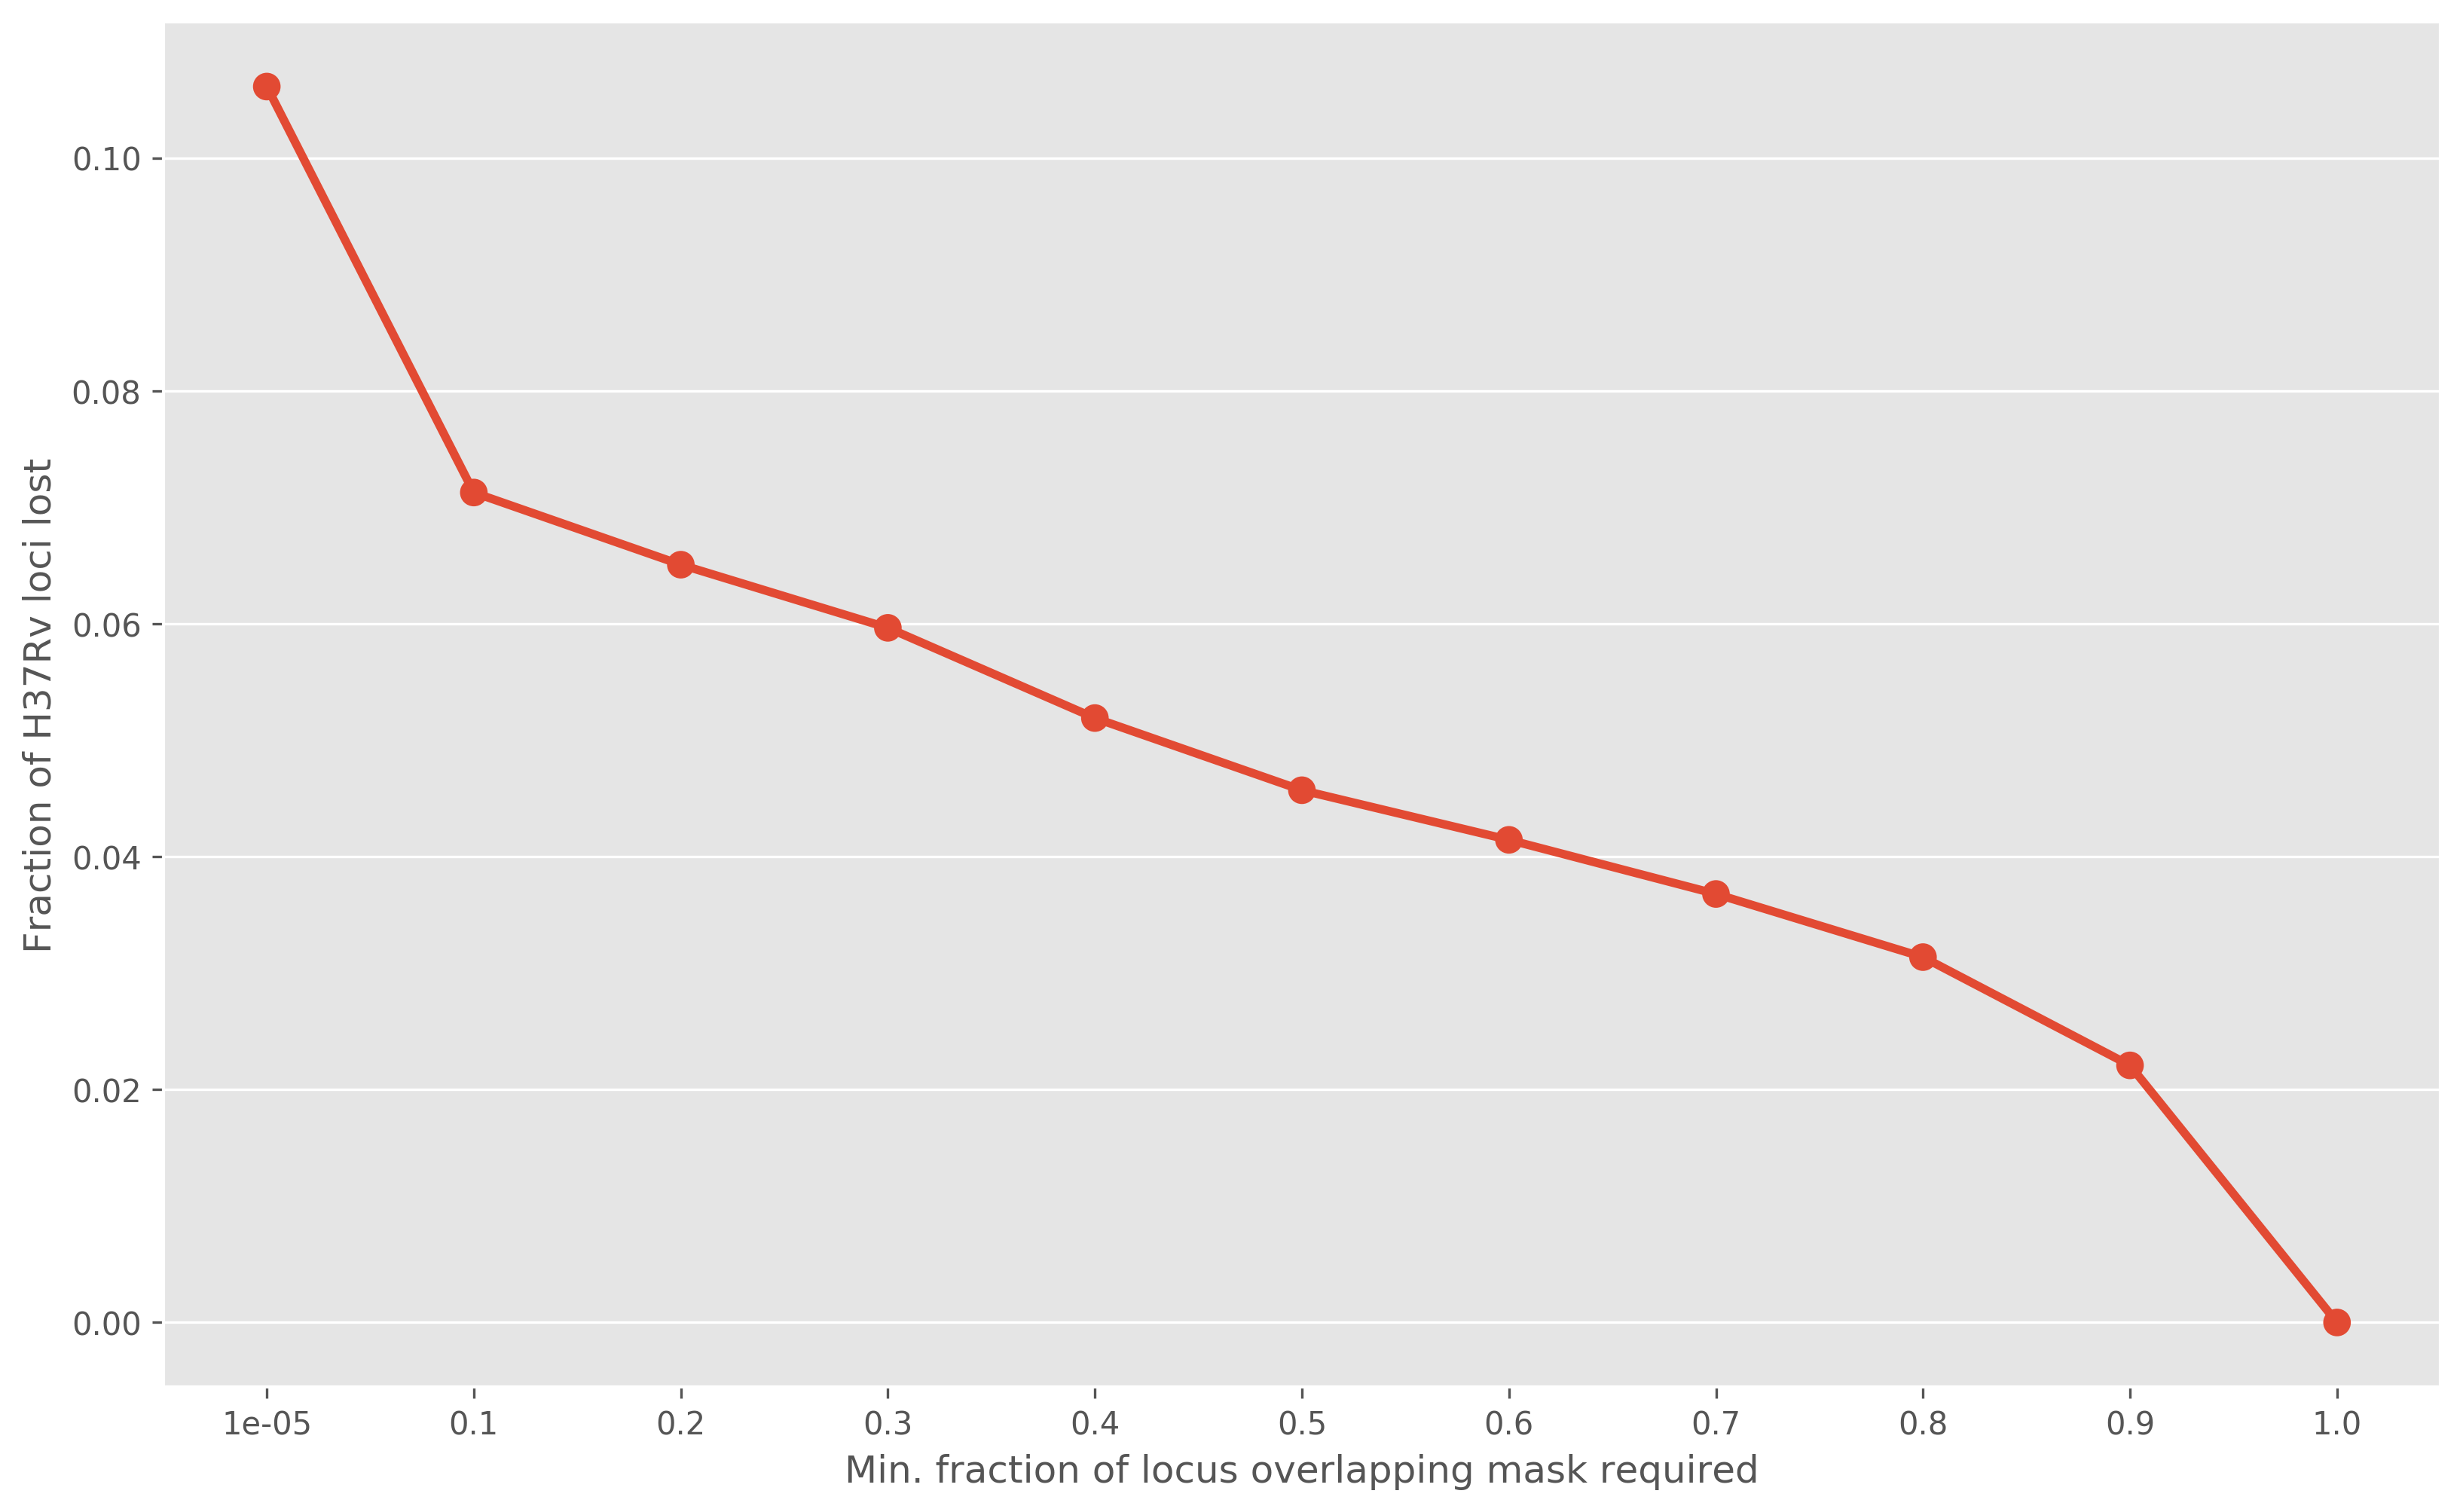
\includegraphics[width=\textwidth]{Appendix1/Figs/loci-lost.png}
         \caption{}
         \label{fig:loci-lost}
     \end{subfigure}
     \hfill
     \begin{subfigure}[b]{0.475\textwidth}
         \centering
         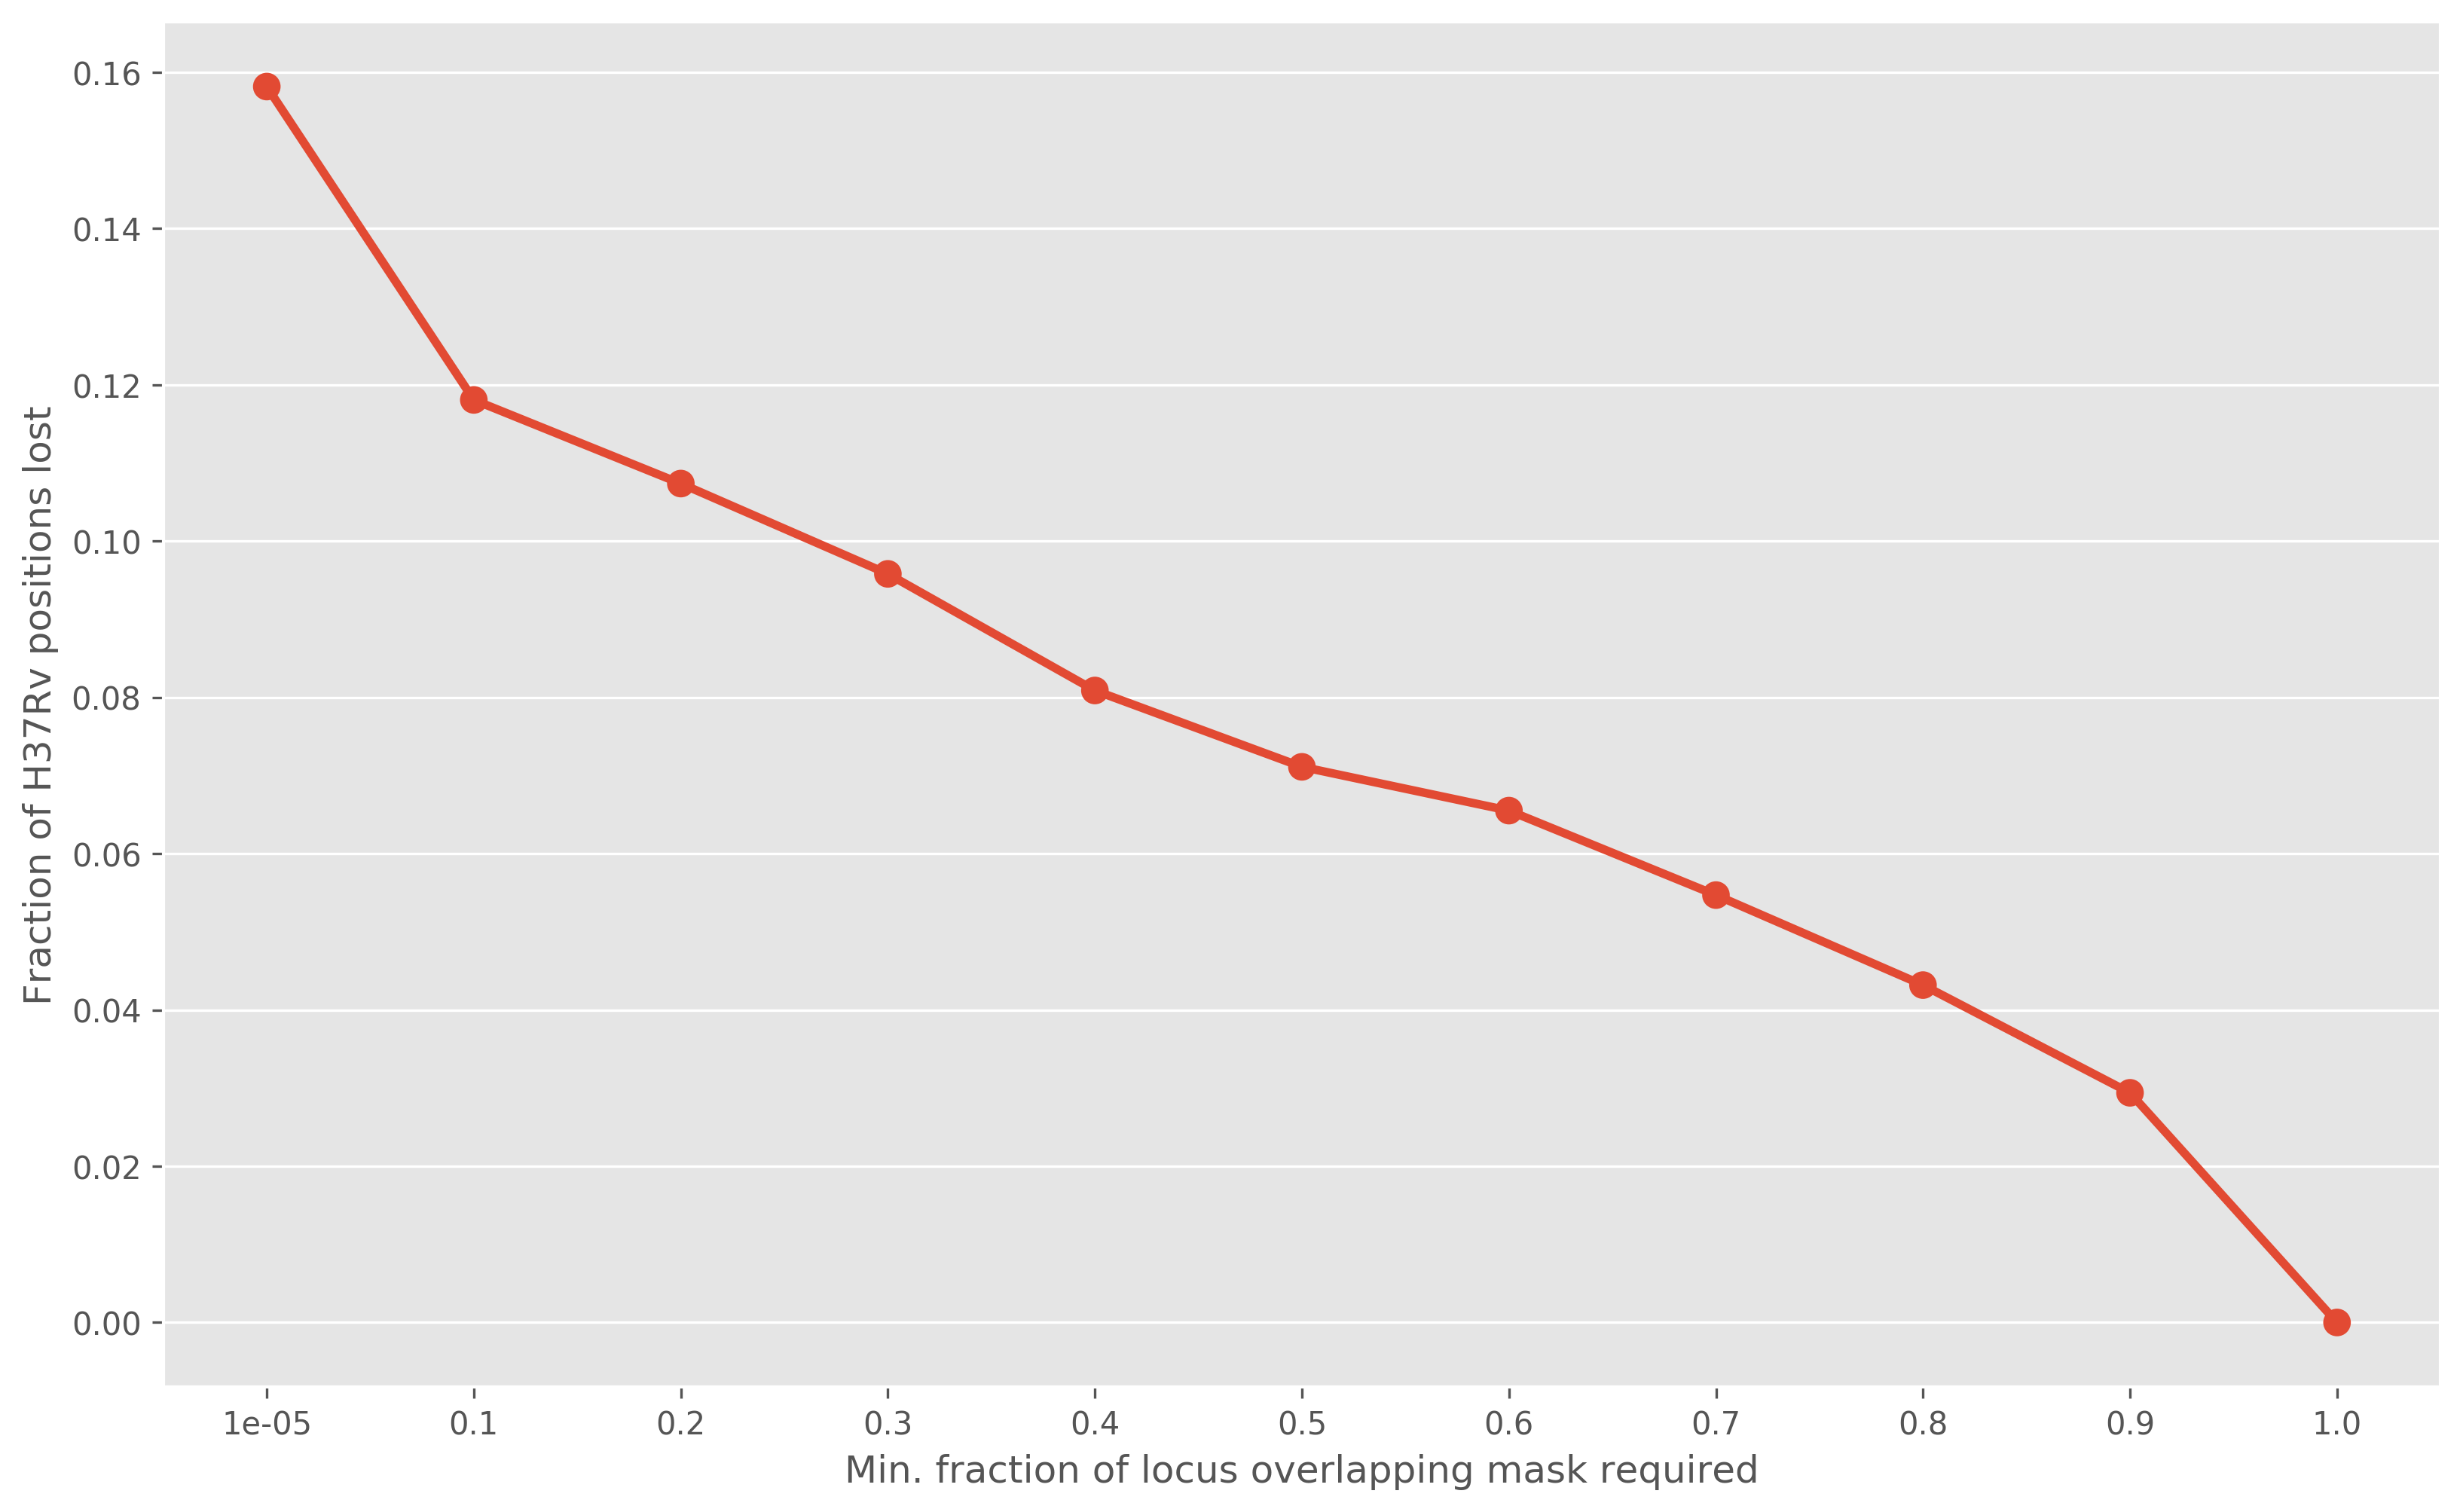
\includegraphics[width=\textwidth]{Appendix1/Figs/pos-lost.png}
         \caption{}
         \label{fig:pos-lost}
     \end{subfigure}
        \caption{\textbf{a)} Proportion of loci lost (y-axis) when removing those with a certain fraction (x-axis) of their positions within the genome mask. \textbf{b)} Proportion of total genome positions lost (y-axis) when removing loci with a certain fraction (x-axis) of their positions within the genome mask.}
        \label{fig:loci-mask}
\end{figure}

% ===========================================================

\section{An illustrated example of clustering similarity metrics}
\label{app:cluster-example}

\autoref{sec:cluster-similarity} outlines three metrics - SACR, SACP and XCR - for evaluating the similarity between two different strategies for transmission clustering. In order to provide the reader with greater intuition for the relevance of each metric, we present an illustrated example in \autoref{fig:cluster-example}. We take \autoref{fig:example-truth} to be the truth clusters and \autoref{fig:example-test} to be some test clusters. These are akin to Illumina and \ont{} clusters, respectively, in \autoref{sec:cluster-similarity}). The individual recall and precision values for each sample in \autoref{fig:example-truth} are shown in \autoref{tab:cluster-example}. SACR and SACP are \emph{sample-averaged}, so their values for this example are 0.82 and 0.83 respectively. To highlight the objective of SACR, we take the truth and test clusters containing the sample $F$. Samples $F$, $G$, $H$ and $I$ are shared between both, but $J$ is missing from the test cluster. To calculate the individual recall for $F$, we take the intersection size of the truth and test clusters it exists in and divide it by that size again, plus the number of samples in the truth cluster that are not in the test cluster - $\frac{4}{5}=0.8$. Ee do the same for the precision of sample $D$, expect we add the number of samples in the test cluster not in the truth cluster to the denominator - giving $\frac{2}{3}=0.66$. The relevance of the XCR metric is best exemplified by the test cluster containing samples $L$ and $M$. As we calculate SACR and SACP for all samples in the truth clusters, these two samples would be ignored. However, they are samples that - according to the truth - should not be part of any cluster. SACR and SACP cannot capture these extra clusterings if they do not contain clustered truth samples. XCR covers this limitation and is the proportion of non-clustered samples (singletons) in the truth that are clustered in the test (see \autoref{eq:xcr}). As \autoref{fig:cluster-example} does not show singletons, let us pretend there are 20 singletons in the truth (including samples $L$ and $M$). This would give an XCR of $2/20=0.1$.

\begin{figure}
     \centering
     \begin{subfigure}[b]{0.4\textwidth}
         \centering
         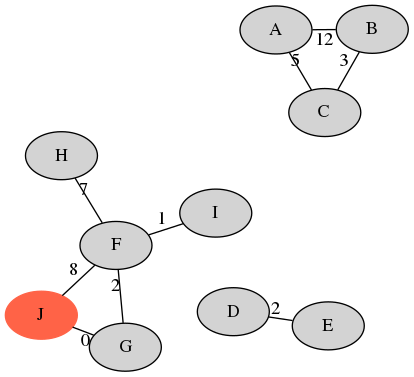
\includegraphics[width=\textwidth]{Appendix1/Figs/illumina-cluster-example.png}
         \caption{}
         \label{fig:example-truth}
     \end{subfigure}
     \hfill
     \begin{subfigure}[b]{0.4\textwidth}
         \centering
         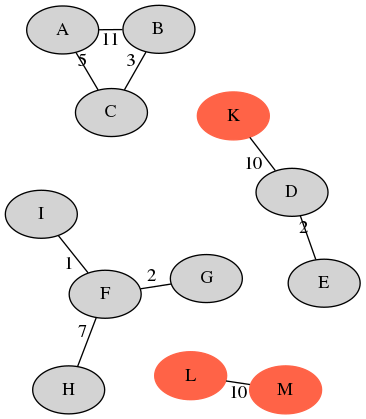
\includegraphics[width=\textwidth]{Appendix1/Figs/ont-cluster-example.png}
         \caption{}
         \label{fig:example-test}
     \end{subfigure}
        \caption{Illustrative examples of transmission clustering. \textbf{a)} represents truth clusters, while \textbf{b)} is clustering from some "test" method we would like to compare to \textbf{a}. The nodes represent samples with the numbers on the edges connecting them indicating the distance between those two samples. The red nodes indicate samples with a clustering disparity between the two clusterings.}
        \label{fig:cluster-example}
\end{figure}

\begin{table}
\centering
\begin{tabular}{|c|c|c|}
sample & recall & precision \\
\hline
A      & 1.0    & 1.0       \\
B      & 1.0    & 1.0       \\
C      & 1.0    & 1.0       \\
D      & 1.0    & 0.66      \\
E      & 1.0    & 0.66      \\
F      & 0.8    & 1.0       \\
G      & 0.8    & 1.0       \\
H      & 0.8    & 1.0       \\
I      & 0.8    & 1.0       \\
J      & 0.0      & 0.0        
\end{tabular}
\caption{Cluster recall and precision results for each sample in \autoref{fig:cluster-example}}
\label{tab:cluster-example}
\end{table}

% ===========================================================

\section{Selecting \ont{} SNP thresholds to define transmission clusters}
\label{app:dist-sweep}

In \autoref{sec:snp-dist}, we found linear models that describe the relationship between the Illumina and \ont{} SNP distance between pairs of samples. Using the equations for each model, we can infer a \ont{} threshold corresponding to a given Illumina threshold. We investigate how well these model-based thresholds perform by using the cluster similarity metrics defined in \autoref{sec:cluster-similarity}. To assess the performance, we by looking at the SACR, SACP, and XCR for all threshold values surrounding the model-based threshold and seeing whether the model-based performs best.

\subsection{bcftools}

For the Illumina SNP thresholds 0, 2, 5, and 12, the corresponding bcftools model-inferred thresholds are 1, 3, 5, and 10 (red vertical dashed lines in \autoref{fig:bcftools-dist-sweep}). Based on the threshold sweep in \autoref{fig:bcftools-dist-sweep}, the best SNP distance thresholds to use for bcftools are deemed 0, 2, 5, and 11 as these provide the best balance between the three similarity metrics.

\begin{figure}
\begin{center}
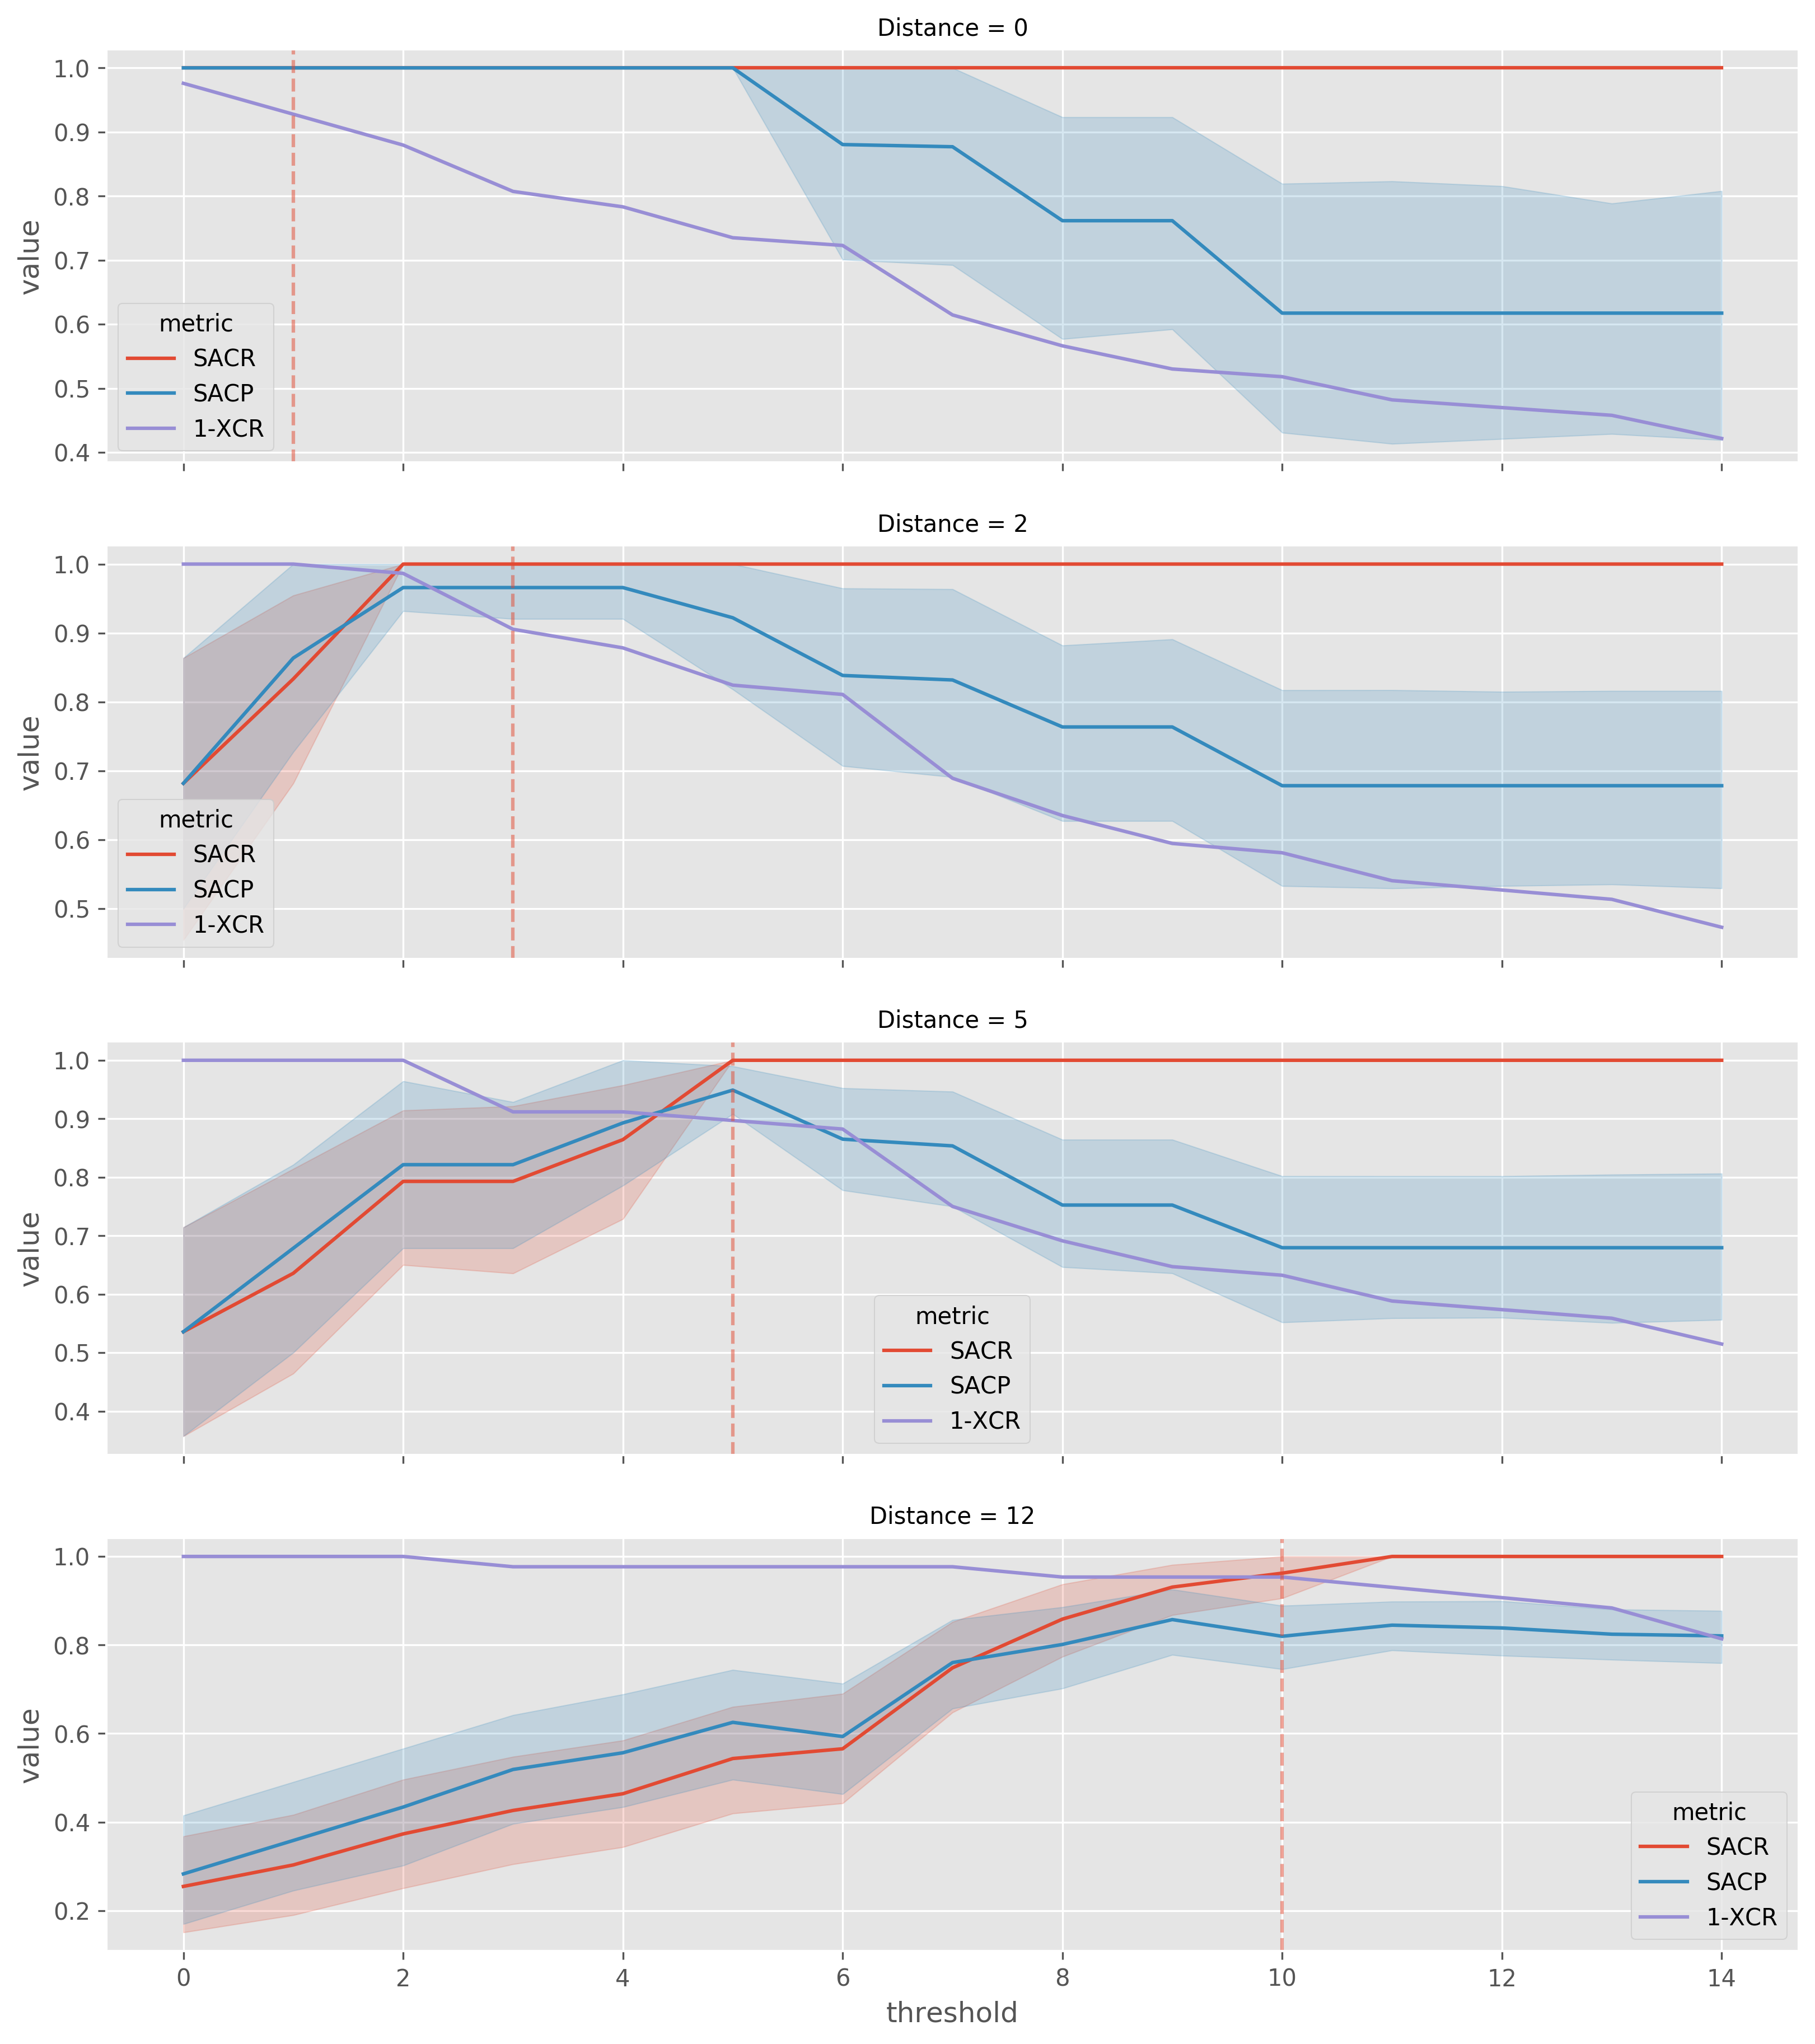
\includegraphics[width=0.90\columnwidth]{Appendix1/Figs/bcftools-threshold-sweep.png}
\caption{{Illumina and \ont{} (bcftools) transmission cluster similarity for various SNP distance threshold. Each subplot compares the \ont{} clustering for the threshold on the x-axis to the Illumina clustering based on the distance (threshold) in the subplot title. SACR (red), SACP (blue), and $1-$XCR are represented by the lines with the band around the line indicating the 95\% confidence interval. The red, vertical, dashed lines indicate the model-based prediction of what the \ont{} SNP distance threshold should be based on the Illumina distance for that subplot.
{\label{fig:bcftools-dist-sweep}}%
}}
\end{center}
\end{figure}

\subsection{\pandora{} single-sample}

For the Illumina SNP thresholds 0, 2, 5, and 12, the corresponding \pandora{} single-sample model-inferred thresholds are 15, 17, 19, and 24 (red vertical dashed lines in \autoref{fig:map-dist-sweep}). Based on the threshold sweep in \autoref{fig:map-dist-sweep}, the best SNP distance thresholds to use for \pandora{} single-sample are deemed 16, 18, 18, and 27 as these provide the best balance between the three similarity metrics.

\begin{figure}
\begin{center}
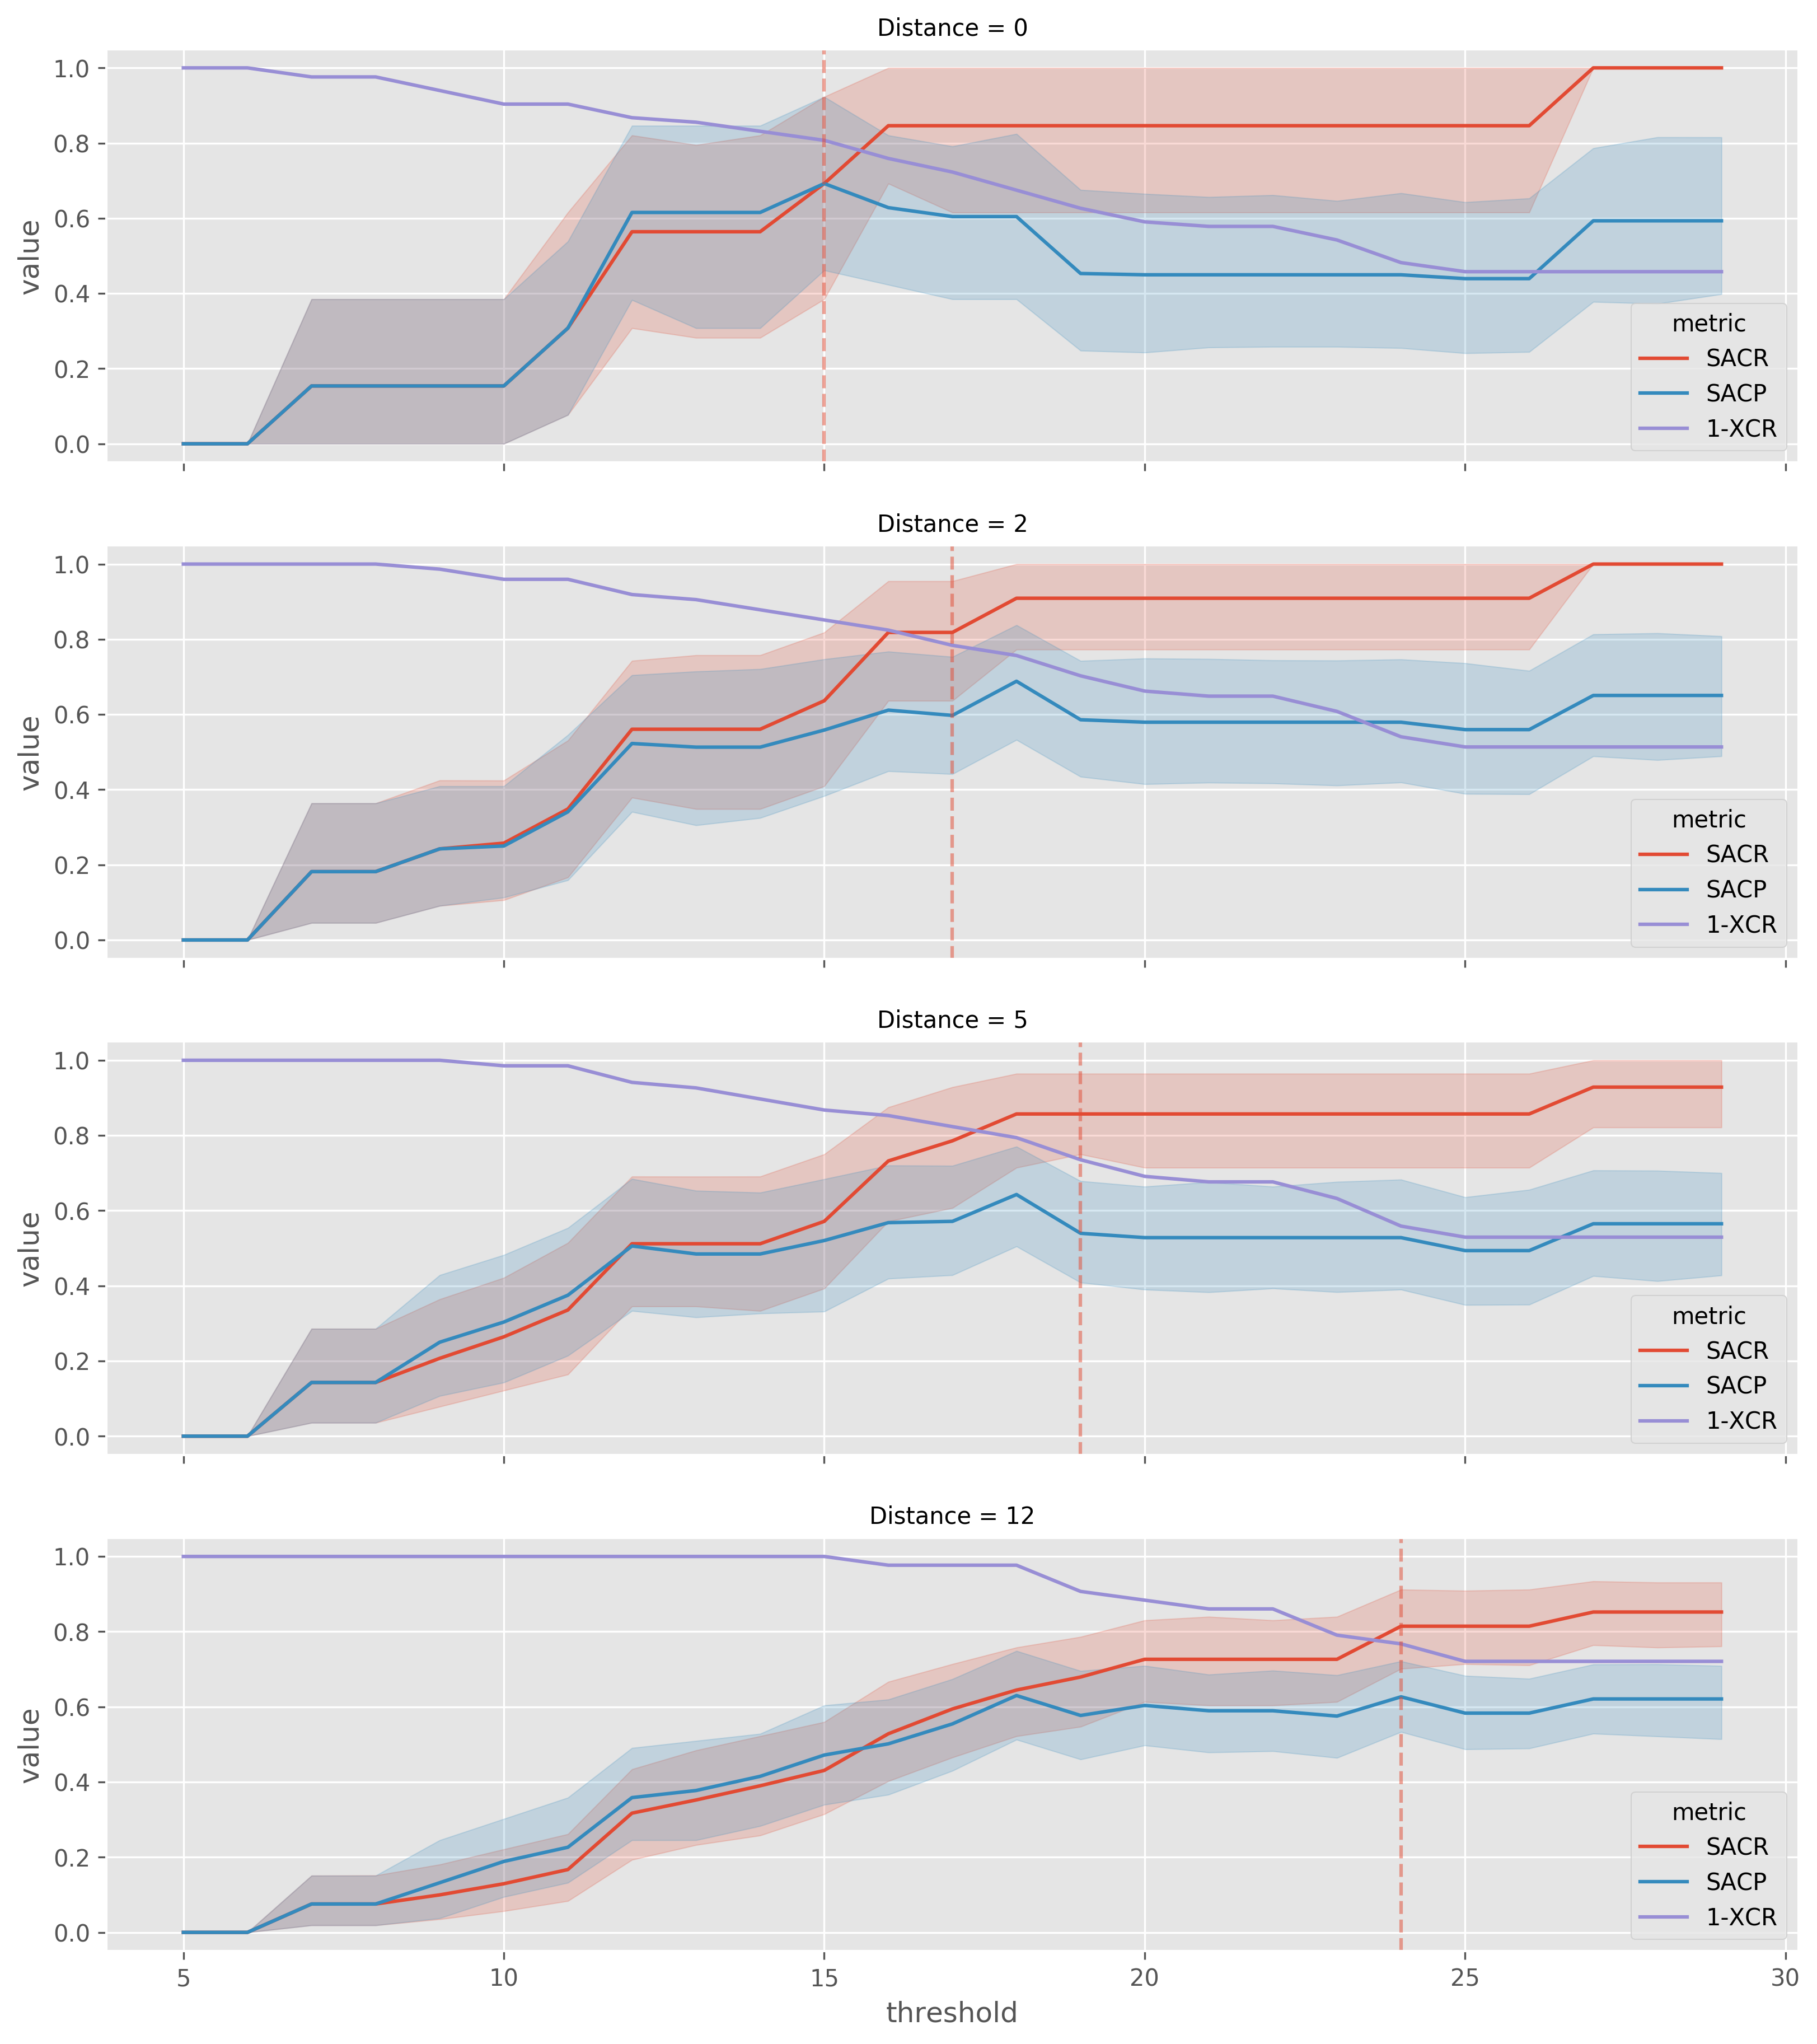
\includegraphics[width=0.90\columnwidth]{Appendix1/Figs/map-threshold-sweep.png}
\caption{{Illumina and \ont{} (\pandora{} single-sample) transmission cluster similarity for various SNP distance threshold. Each subplot compares the \ont{} clustering for the threshold on the x-axis to the Illumina clustering based on the distance (threshold) in the subplot title. SACR (red), SACP (blue), and $1-$XCR are represented by the lines with the band around the line indicating the 95\% confidence interval. The red, vertical, dashed lines indicate the model-based prediction of what the \ont{} SNP distance threshold should be based on the Illumina distance for that subplot.
{\label{fig:map-dist-sweep}}%
}}
\end{center}
\end{figure}

\subsection{\pandora{} multi-sample}

For the Illumina SNP thresholds 0, 2, 5, and 12, the corresponding \pandora{} multi-sample model-inferred thresholds are 0, 0, 1, and 4 (red vertical dashed lines in \autoref{fig:compare-dist-sweep}). Based on the threshold sweep in \autoref{fig:compare-dist-sweep}, the best SNP distance thresholds to use for \pandora{} multi-sample are deemed 0, 1, 3, and 7 as these provide the best balance between the three similarity metrics.

\begin{figure}
\begin{center}
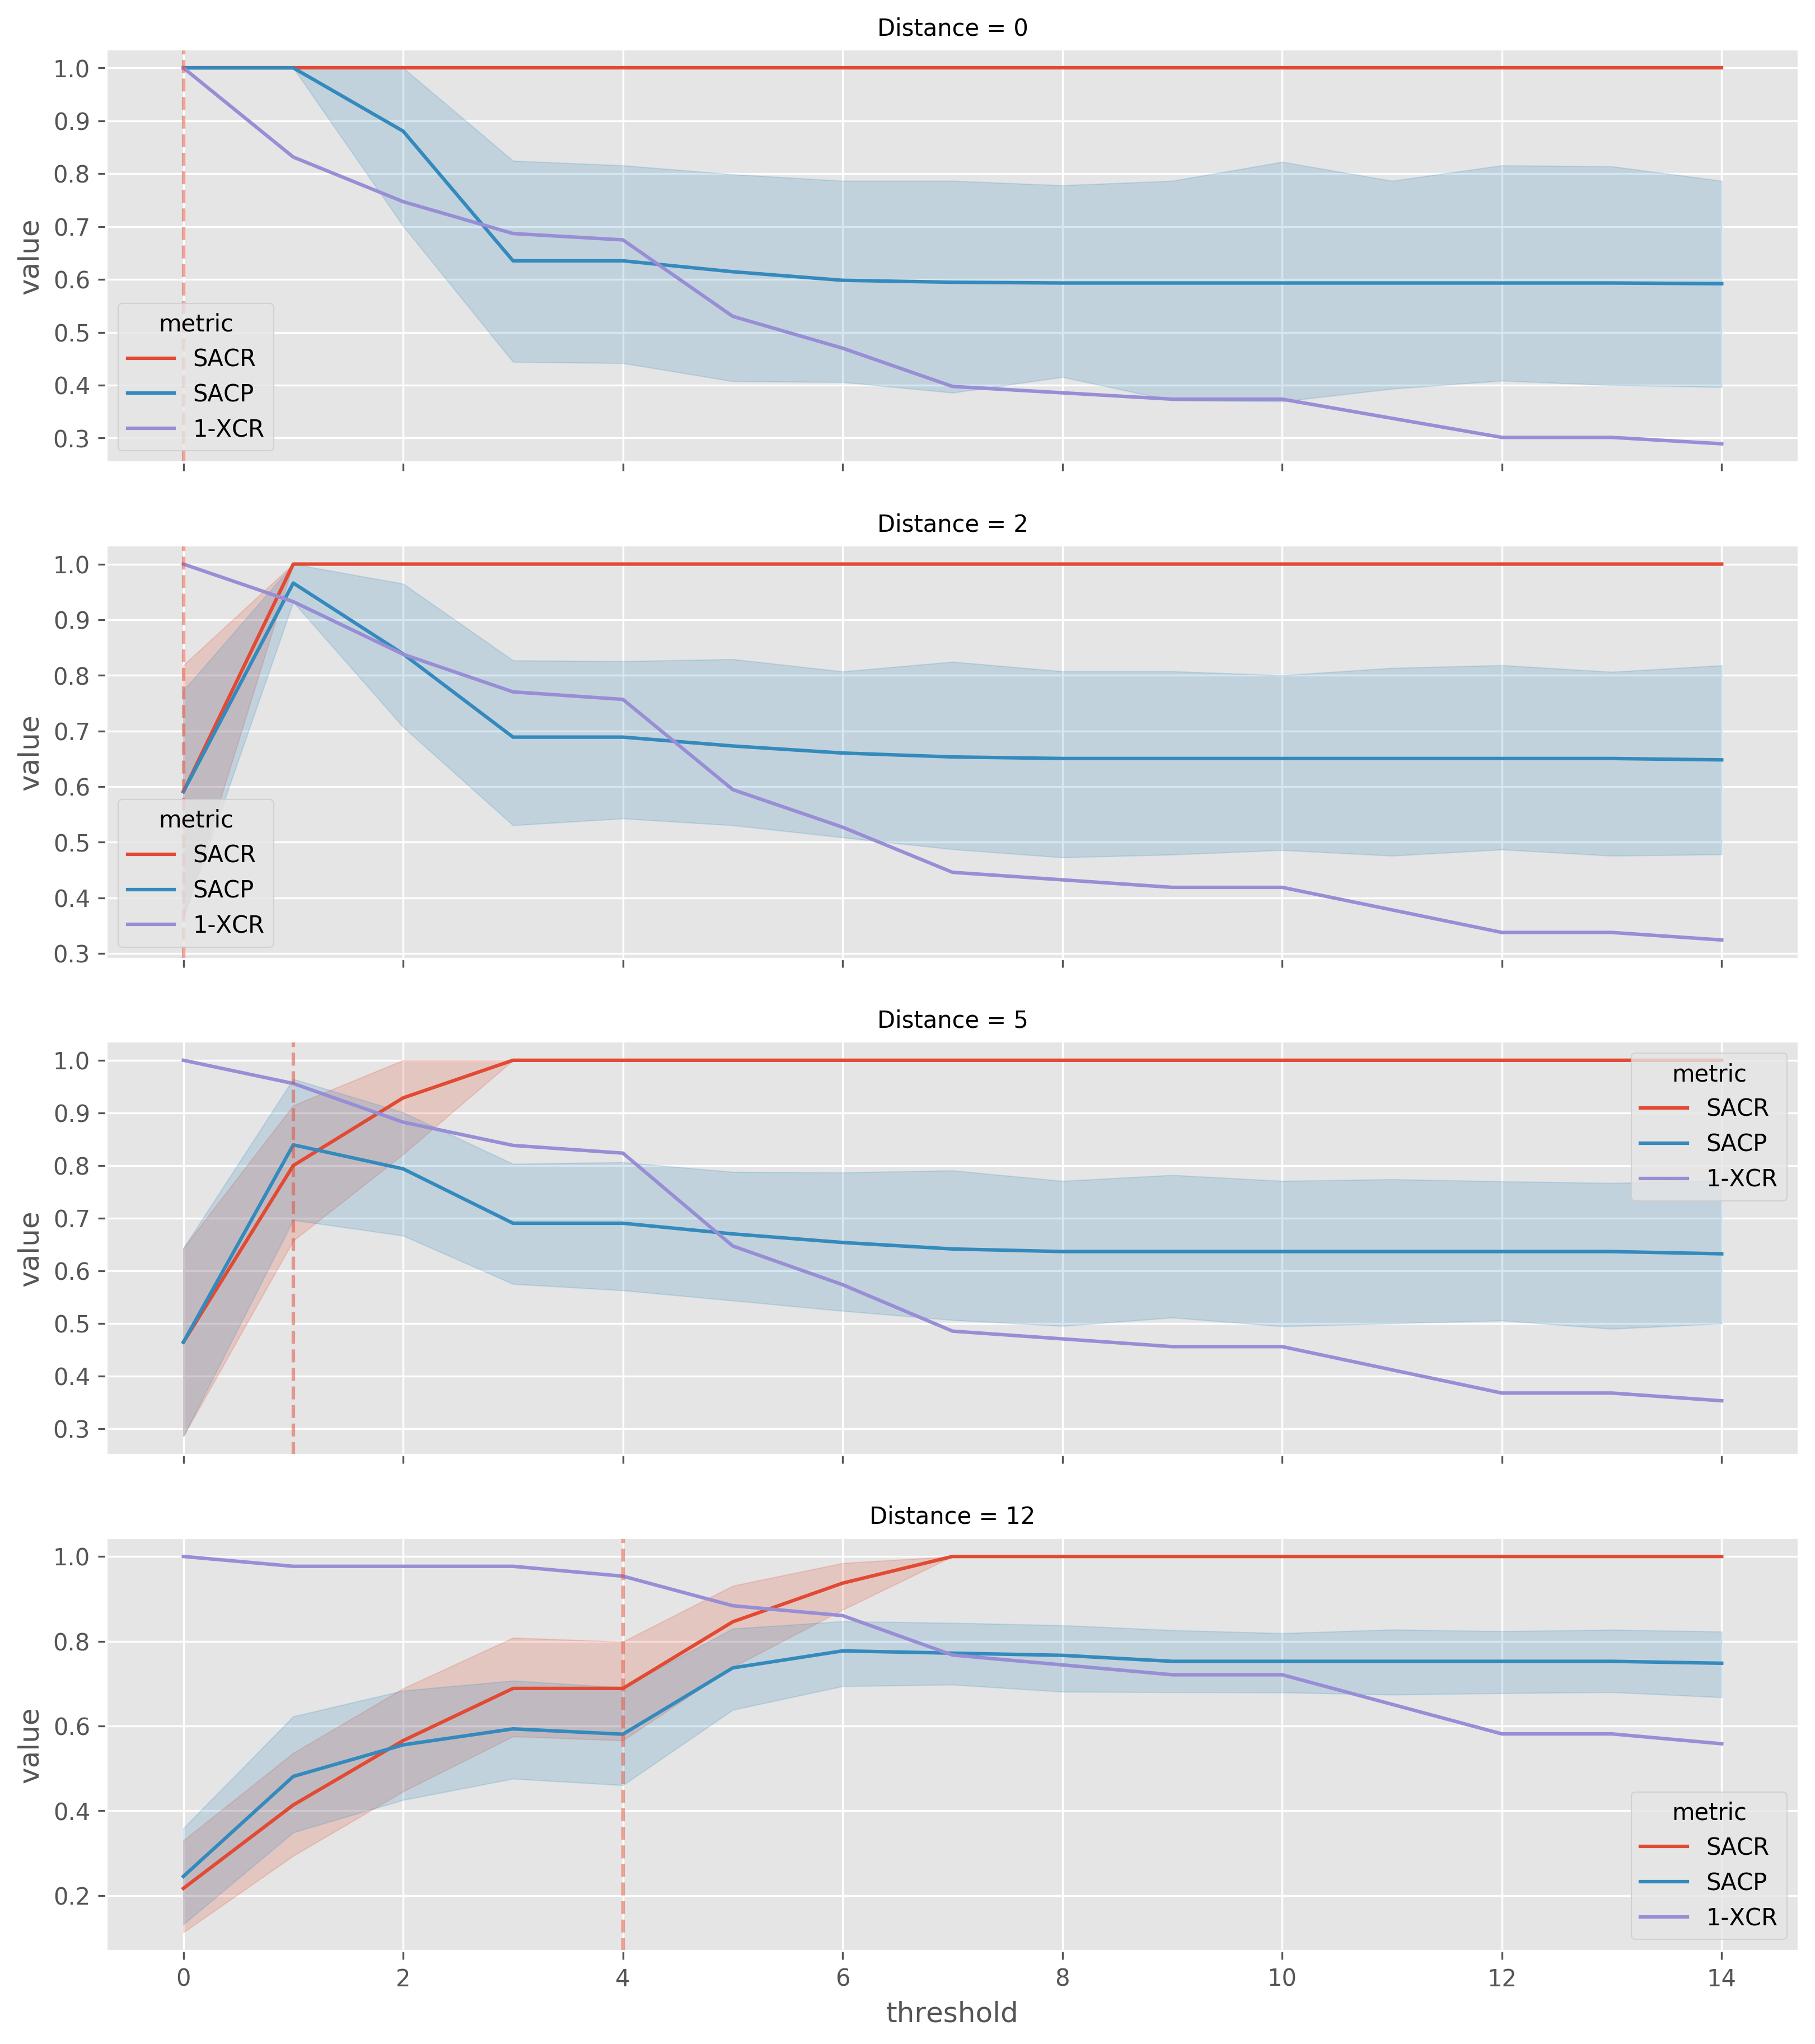
\includegraphics[width=0.90\columnwidth]{Appendix1/Figs/compare-threshold-sweep.png}
\caption{{Illumina and \ont{} (\pandora{} multi-sample) transmission cluster similarity for various SNP distance threshold. Each subplot compares the \ont{} clustering for the threshold on the x-axis to the Illumina clustering based on the distance (threshold) in the subplot title. SACR (red), SACP (blue), and $1-$XCR are represented by the lines with the band around the line indicating the 95\% confidence interval. The red, vertical, dashed lines indicate the model-based prediction of what the \ont{} SNP distance threshold should be based on the Illumina distance for that subplot.
{\label{fig:compare-dist-sweep}}%
}}
\end{center}
\end{figure}

In summary, the model-based thresholds chosen for the \ont{} variant callers are not the best-performing. For all further transmission cluster work, the hand-picked thresholds are used instead.